\section{CUDA 编程教程：向量加法扩展与 GPU 利用率优化}

本章将继续讨论上一个项目。在上一个项目中，处理了两个向量，每个向量包含 1024 个元素，因此选择了一个块和 1024 个线程。本章计划将向量大小扩展到 2048。

\subsection{问题提出与硬件限制}

问题来了：是否可能用一个块来运行 2048 个线程？要回答这个问题，需要查阅白皮书。在 Ampere 架构的情况下，白皮书给出了明确的答案：这是不可能的。每个块的最大线程数是 1024。

\begin{figure}
    \centering
    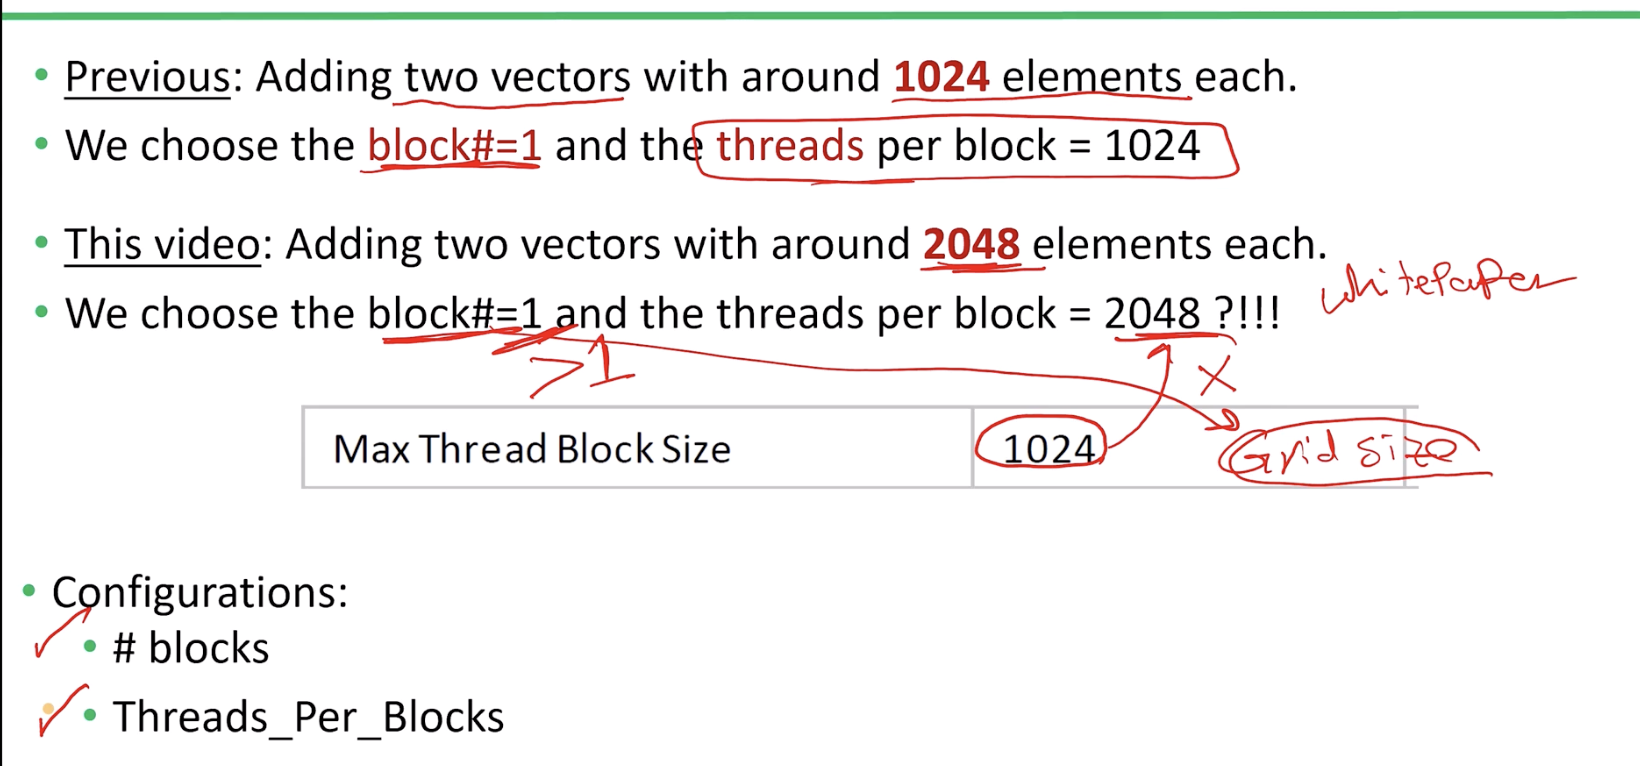
\includegraphics[width=0.75\linewidth]{resources/cuda-077.png}
    \caption{}
    \label{fig:placeholder}
\end{figure}


\subsection{解决方案：调整网格配置}

为了解决这个问题，需要调整网格大小，即增加项目中的块数。与上一个项目使用一个块不同，这里需要使用多个块。可以灵活地决定块的数量以及每个块应包含的线程数，但必须遵循的关键规则是：确保应用程序中的总线程数与向量中的最大元素数相匹配。这意味着如果块数增加（这里的块数指的是网格大小），每个块的线程数必须相应减少，以确保总线程数保持在 2048。

这种情况确实会引起需要关注的性能问题，但将从一个简单的方法开始，只使用两个块，每个块配备 1024 个线程。性能影响将在后续阶段深入探讨。

\subsection{索引映射原理}

如图所示，有一个 2048 个元素的向量。方法是将这个向量分成两部分，每个部分由各自的块来执行。有一个 ID 为 0 的块用于第一部分，一个 ID 为 1 的块用于第二部分。第一部分有 1024 个线程，每个线程专门用于在单个向量元素上执行加法操作，这些线程的 ID 范围从 0 到 1023。这个配置在第二部分中镜像，即第二部分中的线程 ID 范围也是从 0 到 1023。

现在必须将两个部分中的块 ID 和线程 ID 与向量索引对齐，以确保每个向量索引都与一个专用线程匹配来执行加法操作。对于第一部分，这很简单，因为线程 ID 与向量索引相同。然而在第二部分中，向量的索引从 1024 开始，一直到 2047，而线程 ID 仍然从 0 开始，在 1023 结束。

为了解决这个问题，特别是在第二部分，应用以下等式：向量中任何元素的索引计算为\textbf{线程 ID 加上块 ID 乘以每个块的总线程数}。举个例子来验证这个等式对两个部分都有效。

\begin{figure}
    \centering
    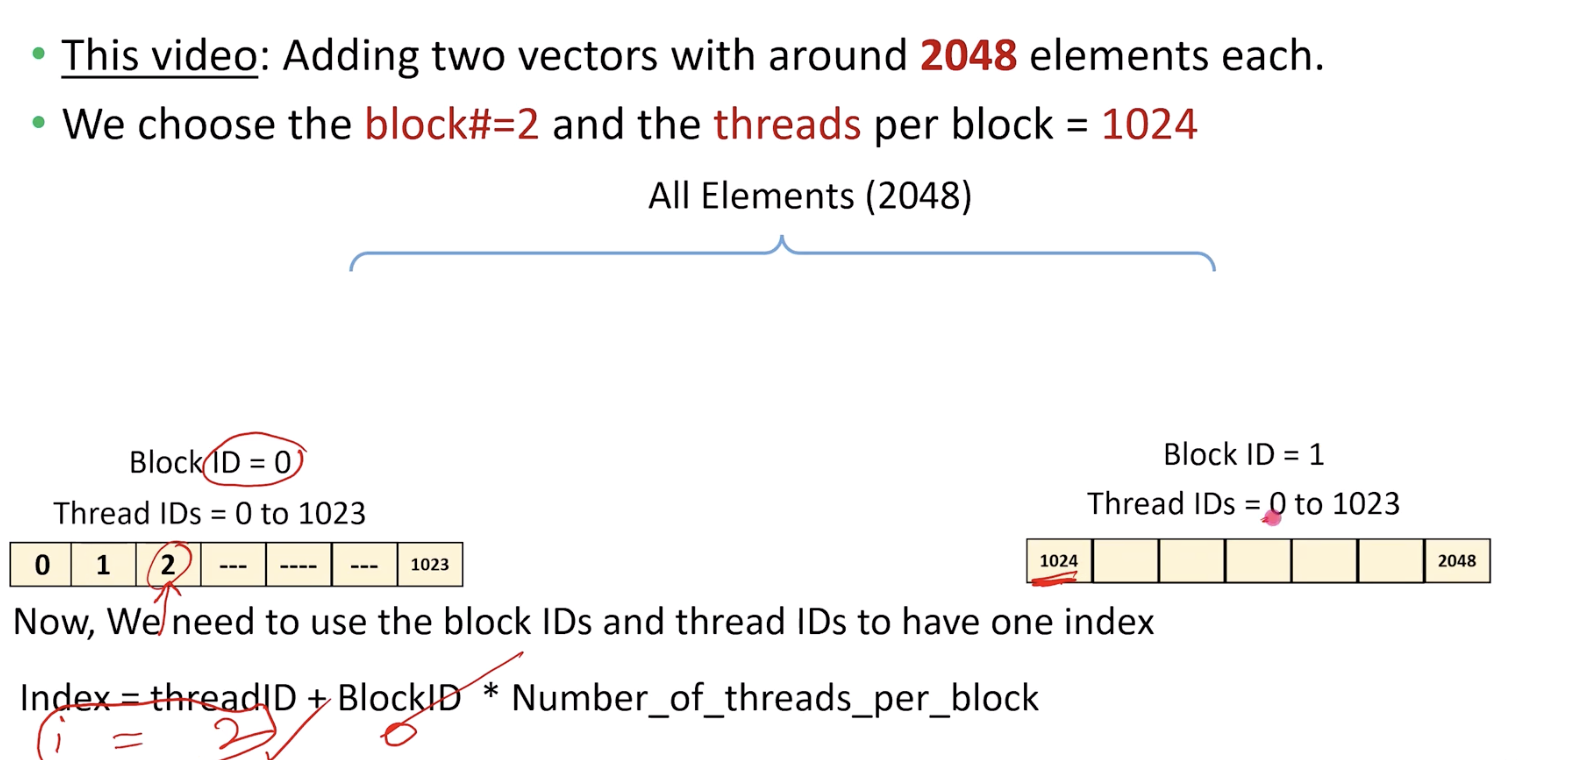
\includegraphics[width=0.75\linewidth]{resources/cuda-078.png}
    \caption{}
    \label{fig:placeholder}
\end{figure}


以向量中的第三个元素为例，块 ID 为 0、线程 ID 为 2。将这些值代入等式，计算结果为索引 2，这是正确的。另一方面，对于后半部分的第一个元素，其线程 ID 为 0，块 ID 为 1，得到索引 1024，这也是准确的。这个等式对两个部分都适用。

需要强调的是，这个等式至关重要，并将继续是 CUDA 编程工作的重要组成部分。

\subsection{代码实现}

请注意，这个等式在编码方面与上一章中的项目非常相似。主要任务涉及直接在核函数中应用索引等式。在这里，将替换这条指令，写成：

\begin{lstlisting}[language=C++,basicstyle=\ttfamily\small]
index = threadIdx.x + blockIdx.x * blockDim.x;
\end{lstlisting}

这里的 \texttt{blockDim.x} 指的是 X 方向上每个块的最大线程数。别忘了在这里将向量大小从 1024 改为 2048。同时需要修改应用程序配置，在这条指令中，需要将这个值从 1 改为 2，以反映对两个块的需求。

在满足其他要求后，现在是编译和运行项目的时候了，并确保每个块中有 1024 个线程。如图所示，项目运行良好，这些就是结果：A 的第一个元素加 B 的第一个元素将存储在 C 向量的第一个位置。

\subsection{GPU 利用率分析}

有两个问题需要探讨，同样的规则适用于 2048 个元素。

\subsubsection{问题一：SM 的使用数量}

第一个问题：基于选择的配置，有多少个 SM（流式多处理器）将被用来执行这个项目？提出这个问题是为了鼓励时刻留意设置对所分配的硬件资源的影响。这将如何影响分配的硬件资源？例如，在这个应用程序中，选择了两个块，每个块 1024 个线程，这将如何影响应用程序的性能？

在回答这个问题时，有必要参考之前提供的图片。如图所示，并且如前所述，一个线程在 GPU 核心上运行（这里的核心是 GPU 中最小的硬件单元，这是软件和硬件中的第二层级）；块在整个 SM 上运行；网格在整个 GPU 上执行。线程束（Warp）在 SM 分区上执行，因为每个 SM 包含多个分区。

据此，在应用程序中，有两个块，这表明只有 2 个 SM 将参与执行这个应用程序。这个衡量标准被称为\textbf{GPU 利用率}。假设拥有 Ampere 架构的 A100 GPU，这个 GPU 拥有 108 个 SM，那么 GPU 利用率将低于总可用 SM 的 2\%。因为只使用了 2 个 SM，而剩下的 106 个 SM 处于空闲状态，没有工作。GPU 利用率是 GPU 性能的一个关键指标。在这个例子中，GPU 利用率极低。

\begin{figure}
    \centering
    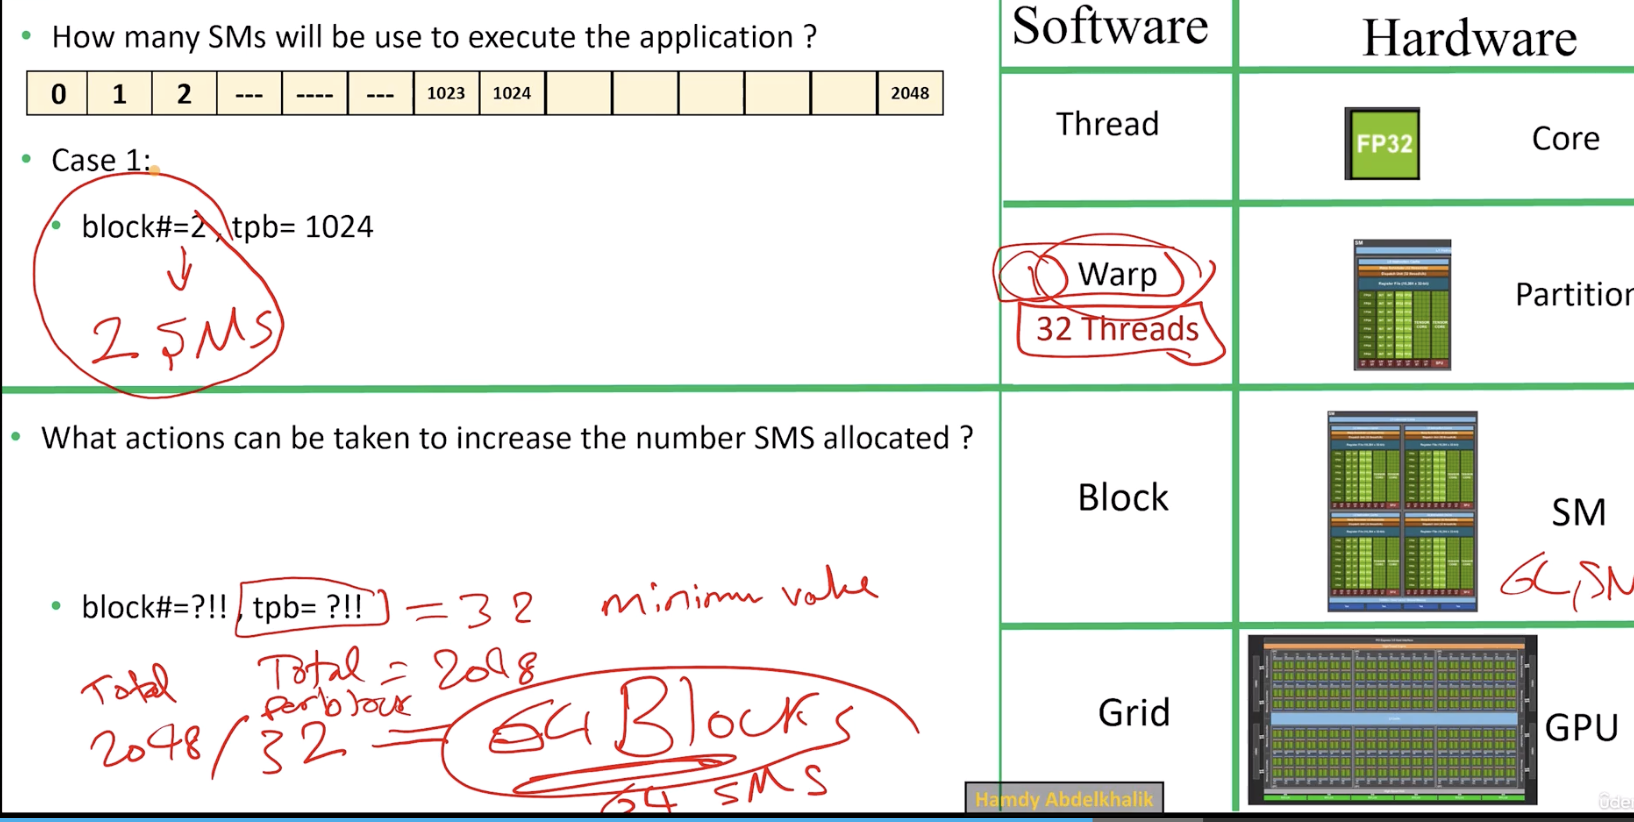
\includegraphics[width=0.75\linewidth]{resources/cuda-079.png}
    \caption{}
    \label{fig:placeholder}
\end{figure}


\subsubsection{问题二：提高 GPU 利用率的措施}

现在看第二个问题：可以采取哪些措施来增加为运行此应用程序分配的 SM 数量？这里希望在不增加向量大小的情况下回答这个问题。这个问题也意味着如何提高 GPU 利用率。

这非常简单：如果能使用更多的 SM，那么就在使用更多的资源，这意味着提高了 GPU 利用率。应该增加块的数量，并且如果可能，应该增加每个块的线程数。在这种特定情况下，同时增加两者不是一个选项，因为总线程数需要与向量中的元素数量匹配。拥有比向量中元素总数更多的线程会引发一个问题：这些额外的线程将执行什么操作？

为了保持总线程数为 2048，策略是增加块数，同时减少每个块的线程数。应该使用的最小每块线程数等于 32，这相当于一个线程束（Warp）的大小，也就是在任何块中可以使用的最小线程数。需要将 2048 个线程除以 32，得到在此应用程序中可以使用的总块数：$2048 \div 32 = 64$ 个块。

这个配置意味着将使用该 GPU（即 A100 GPU）的 64 个 SM。与第一种情况中只有两个块和两个 SM 相比，这里有 64 个块将在 64 个 SM 上运行。

\subsection{执行时间测量}

可以使用两种不同的方法来计算执行时间。为了验证工作并了解这将如何影响应用程序性能，需要测量两种不同场景下的执行时间。一种方法是利用 CUDA 的内置 API，另一种可以使用分析器（Profiler）。本章将采用 CUDA API 方法。这里的分析器指的是 NVIDIA 的诊断工具，如 Nsight Systems 或 Nsight Compute。

现在打开 Visual Studio 看看代码。如图所示，添加了几行专门用于测量执行时间的代码。这个过程的第一条指令是声明两个变量 \texttt{start} 和 \texttt{stop}。之后应用一个名为 \texttt{cudaEventCreate} 的函数。这两个变量是由 \texttt{cudaEvent\_t} 类型声明的，这个函数准备这些变量以供使用，类似于初始化。然后使用 \texttt{cudaEventRecord} 函数来开始记录时间，在这里将初始时间或开始时间存储在 \texttt{start} 变量中。

在这条指令中，正在 GPU 上执行核函数。正如之前讨论的那样，一旦执行完成，再次记录时间并将值存储在 \texttt{stop} 变量中。下一步是使用 \texttt{cudaEventElapsedTime} 函数，从 \texttt{stop} 值中减去 \texttt{start} 值。这个计算提供了以毫秒（ms）为单位的执行时间。

现在编译并运行项目。如图所示，这就是执行时间，请注意这个值。然而再运行一次，读取这个值并记在脑子里。现在再次运行——这印证了对这种计时方法的保留意见。正如观察到的，执行时间可能因每次运行而异。这种方法缺乏精确性，使用分析器是更好的选择。

\subsection{性能对比与总结}

总之，现在回到代码并调整块数和每块线程数。可以在这里选择 64 个块，每个块有 32 个线程，这是第二种场景。再次运行应用程序后，如图所示，可以轻易观察到当前的执行时间比第一种情况减少了。

现在应该清楚了。回到演示幻灯片，更深入地探讨这个话题。

在第一种场景中，有两个块，在总共 108 个可用 SM 中的两个上并行运行。这里需要记住，这些块中的每一个都配置了 1024 个线程，而 1024 个线程是在一个块中可以使用的最大线程数。这意味着这里的块尺寸非常大。

在第二种场景中，有 64 个块在 64 个 SM 上并行运行。与第一种场景相比，这里的块明显更小，每个块包含 32 个线程，而第一种场景中是 1024 个线程。

这里有一个问题：看看第一种情况或第二种情况下可用的 SM，告诉我在任何这些 SM 上将要执行的最大块数是多少。在第一种情况下，第一个 SM 上面将要执行的最大块数是多少？第二个 SM 呢？无论如何，可以说每个 SM 的最大块数等于 1。

再看第二种情况回答同样的问题。有 64 个块，每个 SM 将只执行一个块，这些块将分布在 64 个 SM 上。再次强调，每个 SM 的最大块数等于 1 个块。别忘了这两种情况下的块将并行执行，而不是顺序执行。这意味着执行时间将根据块的大小来计算。如果第二种情况下的块更小，第一种情况下的块更大，那么第二种情况将比第一种情况执行得更快。

希望现在明白了应用程序配置如何影响其性能。本章到此结束。

